\chapter{Astrofísica}

%%%%%%%%%%%%%%%%%%%%%%%%%%%%%%%%%%%%%%%%%%%%%
%%%%%%%%%%%%%%%%%%%%%%%%%%%%%%%%%%%%%%%%%%%%%
%%%%%%%%%%%%%%%%%% SECCION 1 %%%%%%%%%%%%%%%%
%%%%%%%%%%%%%%%%%%%%%%%%%%%%%%%%%%%%%%%%%%%%%
%%%%%%%%%%%%%%%%%%%%%%%%%%%%%%%%%%%%%%%%%%%%%



\section{Introducción: escalas de tiempo y distancia}

\subsection{Historia temporal del Universo}

Los hallazgos de la física de partículas permiten conocer cual era la forma del universo en los primeros instantes tras el Big Bang. Esta historia en los primeros instantes está dividida en diferentes eras, a su vez divididas en épocas y períodos. Los límites que se le dan a estos períodos son estimaciones basadas en los mejores modelos cosmológicos, dando una idea de cual fue el comportamiento en los primeros instantes del universo.

\begin{figure}[h!] \centering
    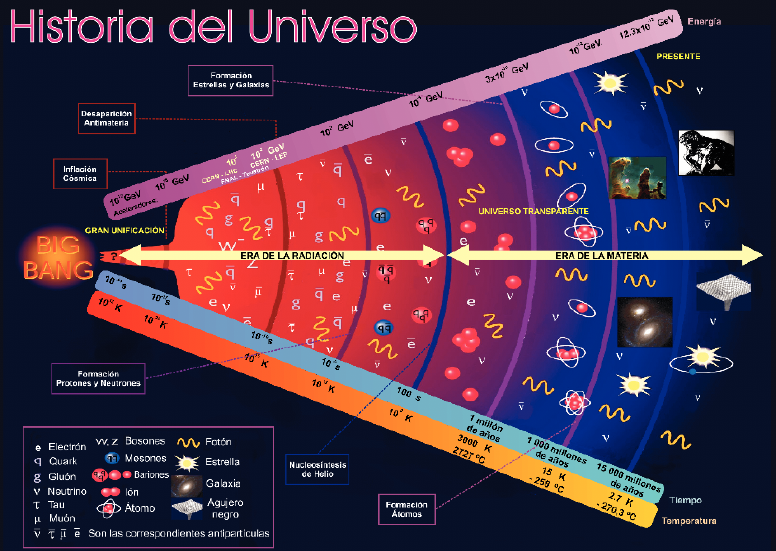
\includegraphics[width=1\linewidth]{Cuerpo/Ch_03/01_Universo.png}
    \caption{Historia del universo.}
\end{figure}
Las eras son 3, a saber:
\begin{itemize}
    \item \textbf{Era de la radiación}: desde el inicio hasta aproximadamente $\SI{4.2e4}{a}$. Debe su nombre a que la mayor parte de la densidad de energía provenía de fotones y neutrinos. 
    \item \textbf{Era de la materia}: desde $\SI{4.2e4}{a}$ a $\SI{2.7e9}{a}$. Debe su nombre a que la mayor parte de la densidad de energía proviene de la materia (protones, neutrones, electrones...) tal y como la conocemos hoy en día.
    \item \textbf{Era de la energía oscura}: desde $\SI{2.7e9}{a}$ al fin del universo. Debe su nombre a que la mayor parte de la densidad de energía proviene de la energía oscura.
\end{itemize}
Nos centraremos en las dos primeras ya que son aquellas que más influencia tienen sobre nosotros. Veamos cuales son las subdivisiones de estas, y cuales son los eventos más interesantes que tienen lugar en esta época. 


\subsection{Escalas de distancias}

Cuando hablamos de longitudes en el unvierso hay que tener en cuenta la gran diferencias en cuanto órdenes de magnitud tanto en distancia de un objeto a otro como en el tamaño de  los objetos. Los objetos con los que trata la astrofísica van desde unos miles de kilómetros $\sim 10^{7}$ m, como exoplanetas; hasta tamaños galáticos o cumulares ($\sim 10^{25}$ m). En cuanto a distancias ocurre lo mismo, alpha centauri (la estrella más cercana) está a unos 3.5 años luz, mientras que solo nuestra galaxia tiene $\sim$200000 años luz de diámetro. 

Por esa misma razón medir distancias es tan complicado, y necesitamos varios métodos en función de lo lejos que esté el objeto y de lo grande que es. En este apartado lo que vamos a hacer es un recorrido desde los métodos para objetos más cercanos hasta aquellos más lejanos. 

\subsubsection{Objetos cercanos: paralaje estelar}

El paralaje estelar es una medida de distancia que nos permite hallar la distancia a la que se encuentran objetos desde aproximadamente a $1/5$ kpc (estos últimos con una gran incertidimbre). 

\subsubsection{Magnitudes aparences, absolutas y relación con la distancia}

Podemos usar el brillo de las estrellas/objetos para calcular la distancia a la que están los objetos. Sin embargo, existe un problema que hay que solventar: no todas las estrellas brillan igual, y por tanto la luminosidad como tal no es una magnitud, por si sola, buena para obtener distancias. 


\subsubsection{Escalas Galácticas y extragalácticas}

Existen otras maneras que permiten las distancias cuando ya no funciona el paralaje. Los métodos se van solapando en una escalera de distancas cósmicas mediante la utilzación de candelas estándar, objetos que tienen luminosidad $L$ conocida o una característica que permite usarlas para medir la distancia en función del flujo observado. A escala galáctica tendremos:

\begin{itemize}
    \item \textit{Paralaje dinámico de estrellas binarias}.
    \item \textit{Variables Cefeida}. 
    \item \textit{Variables RR Lyrae}.
    \item \textit{Paralaje espectroscópico}.
    \item \textit{Binarias eclipsantes}.
\end{itemize}
Para completar la escalera de distancas cósmicas tenemos las escalas extragalácticas:

\begin{itemize} 
    \item \textit{Candela estelar}. Son cefeidas que se pueden detectar, sobretodo las más luminosas.
    \item \textit{Características comúns}. Podemos supoenr que algunos cúmulos son parecidos a los que ya conocemos y relacionar entonces la luminosdidad vista con la distancia.
    \item \textit{Supernovas tipo I}. Este es el método que más se usa junto con el corrimiento al rojo. Usa las violentas explosiones de supernovas, de las cuales conocemos el brillo esperado, para poder determinar cuan lejos está. 
    \item \textit{Corrimiento al rojo}.
\end{itemize}


\subsection{Escalas galácticas: estrellas binarias}

Las estrellas dobles o binarias son pares de estrellas que orbitan alrededor del centro común de masas. Estímase que la mitad de las estrellas observables en el cielo agrúpanse en estrellas binarioas o sistemas múltiples. El estudio de las estrellas binarias permite calcular la masa y radios estelares y lasd istancias relativas de las estrellas, mediante procedimientos básicos de determinación de elementos orbitales. 

\begin{itemize}
    \item Binarias visuales: las dos estrellas son detectables opticamente y sus elementos orbitaels pueden determinarse a través de observaiones seperaadas en el tiempo. Coñecese alrededor de mil setecientos binarias visuales.
    \item Binarias astrométricas: solo una de las estrellas es visible (por ejemplo una gigante roja y una estrella de neutrones, una será visible y otra no, pero la masa será similar, lo que hace que orbiten respecto un centro de masas, lo que si permitirá detectarlas, pero solo con el movimiento oscilatorio).
    \item Binarias eclipsantes: si las estrellas están orientadas con su plano orbital en la línea de visión cara la tierra, la curvatura de luz detectada mostrará variaciones (mínimos) periódicos cuando una de las estrellas eclipse total o parcialmente a la luz de la compañera. En muchas ocasiones permite medir las deformaciones y distorsiones o incluso la transferencia de masa entre estrellas. 
    \item Binarias especcrtrales: en la media del espectro de las estrellas se observa características que corresponden a dos tipos de espectralesdiferentes, en ocasiones con corrimientos Doppler diferentes
    \item Binarias espectroscópicas: las líena espectrales de cada componente del par se desplazan en diferente sentido (cara azul o rojo) alterantivamente. 
\end{itemize}
Esta clasificación no es mutuamente exclusiva: ciertas binarias se estudian por diferentes procedimientos. La primera ley de kepler nos dice que todos los objetos en una línea vinaria se mueve alrededor del centro de masas en órbitas elípticas, siendo el centro de masa uno de los focos de la elipse. La segunda ley de Kepler nos dice que el radio vcto entre dos objetos en órbita y el centro de masa recorre áreas iguales en tiempos iguales 

\begin{equation*}
    \derivadas{A}{t} = \frac{1}{2} \frac{L}{\mu}
\end{equation*}
La tercera ley de kepler nos dice que el cuadrado del período orbital es directamente proporcional al cubo de la longitud del semieje mayor de la órbita elíptica alrededor del centro de masa e inversamente propircional a la masa total del sistema. 

\begin{equation*}
    P^2 = \frac{4\pi^2}{G(m_1+m_2)} a^3
\end{equation*}
Partiendo de los elementos orbitales del par de estrellas se puede determinar el \textbf{coceinte de las masas}. Para este cálculo tenemos qeu determinar el plano orbital y proyectar las observaciones en ese plano, por definición del centro de masas. 

\begin{equation*}
    \frac{m_1}{m_2} = \frac{a_2}{a_1}
\end{equation*}
Existe una clara relación entre la medida de la masa y la luminosidad (en magnitudes absolutas o en normalizada a Sol). Nótese que la escala logarítmica en ambos casos y en ambos ejes (la magnitud es una escala logarítmica). Más adelante veremos qeu esto fue uno de los indicativos para construir el diagrama de Herzsprung-Russel (luminosidad-temperatura).

\subsection{Composición del Universo y el Sistema Solar}

El orgen de los elementos en la creación del sistema solar: el sistema solar se formo a partir del colapso de una nebulosa gaseosa con abundancias químicas e isotópicas uniformes y coincidentes con las observadas en otras partes del universo (obtenidas mediante mediciones espectroscópicas, granos presolares en meteoritos primitivos). Las abundancias químicas se obtiene la forma independiente y complementaria:

\begin{itemize}
    \item Observacioens de la fotoesfera solar.
    \item Análisis de una clase particular de meteoritos.
\end{itemize}



%%%%%%%%%%%%%%%%%%%%%%%%%%%%%%%%%%%%%%%%%%%%%
%%%%%%%%%%%%%%%%%%%%%%%%%%%%%%%%%%%%%%%%%%%%%
%%%%%%%%%%%%%%%%%% SECCION 2 %%%%%%%%%%%%%%%%
%%%%%%%%%%%%%%%%%%%%%%%%%%%%%%%%%%%%%%%%%%%%%
%%%%%%%%%%%%%%%%%%%%%%%%%%%%%%%%%%%%%%%%%%%%%


\section{Teoría de la radiación}

\subsection{Propiedades corpusculares de la radiación}

Para explicar el cuerpo negro es improtante recordar las siguiente deficiones y conceptos: 

\begin{itemize}
    \item Radiación térmica: la emitida por un cuerpo como consecuencia de su temperatura.
    \item Cuerpo negro: emisor ideal, aquel cuya superifice abosrbe toda radiación que incide sobre él.
    \item Radiación espectral: energía emitida en forma de radiación por un cuerpo negro a una temperatura $T$ constante, con frecuencia en el intervalo ($v$,$v+\D v$), por unidad de ángulo sólido, área proyectada y tiempo. 
\end{itemize}
A finales del siglo XIX las observaciones de los espectros térmicos no concordaban con con las prediciones:

\begin{itemize}
    \item Ley de Stefan-Boltzman. La referencia total emiitda por $B_T = \sigma T^4$. 
    \item Ley del desplazamiento de Wien. $\lambda_{\max} = C / T$ siendo $C$ una constante y $\lambda_{\max}$ es la longitud de onda del máximo de $B(\lambda)$. 
    \item Teoría de Plank: la densidad de energía (energía por volujmen y longitud de onda/frecuencia) en una caja es:
    \begin{equation}
        \rho_\tau (\lambda) \D \lambda = \frac{8 \pi \hbar c^2}{\lambda^5} \frac{\D \lambda}{e^{hc/k_BT}-1}
    \end{equation}
    qeu se deduce a partir del postulado de Plank: los entes físicos con un grado de liberatad, dode su coordenada característica es función sinosuidal con el timepo, solo pueden tener energías totales cuantizadas, según $E=n h \nu$ con $n=1,2,3...$ El ajuste de los datos experimentales con la teoría es impresionante. 
\end{itemize}

\subsection{Aplicaciones astrofísicas}

La radiancia espectrtal (intensidad de radiación o energía por unidad de área, tiempo y ángulo sólidio emitida en el rango de una longiturd de onda entre $\lambda$ y $\lambda + \D \lambda$). Una vez integrada podemos obtener la luminosidad:

\begin{equation}
    L = 4 \pi R^2 \sigma T^4_e
\end{equation}

\subsection{Espectros atómicos}

Los átomos pueden estar en diferentes estados de ionización con espectros característicos diferenciaddos. Los espectroes observadores correspodnen a sistemas gaseosos en equilibrio local. En particular, a ua t empreatura $T$ dada, el cociente de posibildia de ocupación d los estados $a$ y $b$ con degernación  $g_a$ y $g_b$ vendrá dada por el \textit{factor de Boltzmann}: 

\begin{equation}
    \frac{N_b}{N_a} \simeq \frac{P(S_b)}{P(S_a)} = \frac{g_b}{g_a} e^{-(E_a-E_b)/k_BT}
\end{equation}
De las relaciones entre las diferentes entre las energías de los estados y de la tempratura podremos obtener el cociente de las ocupaciones de cadda uno de los estados accesibles. Es preciso hacer un cálculo cuántico riguroso para determinar la degenración $g$ de un estado determinado. 

La ecuación de Saha calcula el grado de ionización del gas cuando está en equlibrio térmico a partir de la funión de partición para cada estado ionizado. El cocientre enter el número de átomos en cada posible estado ionizado viene dado por:

\begin{equation}
    \frac{N_{i+1}}{N_i} = \frac{2Z_{i+1}}{n_eZ_i} \parentesis{\frac{2\pi m_eK_B T}{\hbar^2}}^{3/2} e^{-\frac{x_i}{kT}}
\end{equation}
donde $n_e$ es la densidad numérica de elctrones libres, y la función de partición $Z_i$ para lelgar al estado ionizado:

\begin{equation}
    Z_i = \sum_{j=0}^\infty g_j e^{-(E_j-E_i)/kT}
\end{equation}
Con todo, el significado de las leyes espectroscópicas de Krichoff para la astrofíscia ahora resultan evidentes:

\begin{itemize}
    \item Un gas denso y caliente o un objeto sólido produce un espectro continuo de radiaciíon de acuerdo con la emisión de un cuerpo negro para una determianda tempratura, descrito por la raidanza espectral descrita por Plank.
    \item Un gas difuso produce líneas de emisión birllantes cuando se producen transiciones de electrones de una órbita a otra mas ligada. Las relaciones se Saha y Boltzmann permiten avaliar la itensidade relativa entre líneas tanto en los espectros de emisión como en los de absorción.
    \item Un gas difuso más frío qeu una fuente espectral captura de lso fotones y ciertas(...)
    \item (...)
\end{itemize}

\subsection{Efecto doppler}

El \textbf{corrimiento Doppler} se produce cuando un movimiento del emisor de una onda modifica la longitud de onda observada. Llamando $v_f$ a la velocidad radial entre emisión y receptor $v_s$ a la velocidad de trasmisión de la onda en el medio:

\begin{equation}
    \frac{\lambda_{obs}-\lambda_{rest}}{\lambda_{rest}} = \frac{v_r}{v_s}
\end{equation}
Esta relación es válida para ondas de sonido, pero no se puede aplciar a la luz. Para la luz necesitamos una formualción relativista que tenga en cuenta la dilatación temporal relativista y la distancai adicional que percorre la luz. Si la fuente se mueve, respecto al observador, $u$ ($\beta=u/c$) y la luz se emite entre los tiempos $t_1$ y $t_2=t_1+\Delta t$:

\begin{equation}
    \Delta t = \frac{\Delta t_{rest}}{\sqrt{1-\beta^2}}
\end{equation}
Teniendo que tener en cuenta el incremrento de la distancia:

\begin{equation}
    \Delta D = \frac{u\Delta t_{rest}\cos(\theta)}{\sqrt{1-\beta^2}}
\end{equation}
Con todo, el efecto global es:

\begin{equation}
    \Delta t_{obs} = \frac{\Delta_{rest}}{\sqrt{1-\beta^2}}(1+\beta \cos (\theta))
\end{equation}

El corrimiento Doppler relativista se obtiene de la diferencia temporal $\Delta t_{obs}$. Aplicándolas para determinar las frecuencias según el observador:

\begin{equation}
    v_{obs} = \frac{v_{rest}}{\gamma(1+\beta \cos (\theta))}
\end{equation}
para el desplazamiento radial:

\begin{equation}
    v_{obs} = v_{res} \sqrt{\frac{1-\beta}{1+\beta}}
\end{equation}
Observamos un desplazmaiento al rojo de las longitudesde onda cuando los objetos que meiten la luz se lejan a altas velcoidades de nosotros, de igual forma, en el caso de acercaser, veríamos un desplazamiento al azul. Definimos el parmaétro $z$ como el \textbf{parámetro del corrimiento al rojo} como:

\begin{equation}
    z = \frac{\Delta \lambda}{\lambda_{res}}
\end{equation}
Los efectos tienen que tener en cuenta las variaciones de las frecuencias de las líneas espectrales observadas pero tamibén en los efectos periódicos, en los que ha que calcular el tiempo propio del sistema qeu recede. El parámetro $z$ del corrimento al rojo puede venir motivado por el corrimiento doppler relativista, pero también por la meisión de radiación en un campo gravitatorio (corrimiento al rojo gravitacional) y también por la expansión propia del Universo (corrimiento al rojo cosmológico). 

\subsection{Tipos espetrales de las estrellas}

La clasificación moderna de Harvadr o Morgan-Keenan asigna letras a lso tipos espctrales en una secuencia decreciente de temperaturas: O, B, A, F, G, K, M, L, T. Cdaa clase posee subdivisiones (10, del 0 al 9) en función las características que paulatinamente se van suciediendo. Existen otras clases (D,S,C) para espectros de estrellas especiales que no se enmarcan en la categorización anterior. De forma adicional (veremos más adelante el diagrama HR y su importancia), diferntes características de espectros diferentes entrellas que llevan a añadir:


\begin{itemize}
    \item 0 o Ia+: hipergigantes o supergigantes estremadamente luminosas.
    \item Ia: supergigantes muy luminosas.
    \item Iab: supergigantes luminosas de tamaño intermedio.
    \item Ib: supergigantes menos luminosas.
    \item II: gigantes brillantes.
    \item III:
\end{itemize}
Hay muchos detalles más que a veces aparecen como subíndices, notas, paréntesis...  Además hay clases adicionales para estrellas especiales novas o que no entran bien en la categoriazación: W (tipo Wolf-Rayet), L, T, Y (especroes infrarrojos), estrellas con carbón (C-R,C-J,C-H,C-Hd) clase $S$ similar a la $M$ pero con fuertes líneas de absorción de ZrO, y clases P y Q para objetos estelares. Además una completa caracterización para las ennanas blancas. 

\subsubsection{Tipo O}

El tipo O son gigantes (más de 16 masas solares) azules, extremadamente calientes ($3.3\times 10^4$ K) y luminosas, que radian ampliamente en el UV. Son escassas pero comprenden alguna de las estrellas más conocidas. Tienen líneas de absorción dominantes para el He II. Son estrellas que no tienen atmósferas grandes debido al viento estelar que producen. Tienen enormes cores calientes y quemddan de forma rápida su hidrógeno, qeudando poco tiempo en la secuencia princicpal.

\subsubsection{Tipo B}

Son estrellas calientes ($1-3.3 \times 10^4$ K) azules de tamaño medio-gradne (mas de dos masas solares), muy luminosas. El $0.125\%$ de las estrellas en la secuencia principal son del tipo A.

\subsubsection{Tipo A}

Son estrellas blancas-azuladas calientes (7500-10000 K), grandes (del promedio de dos masas solares, de 1 a 15) cuando están en la secuencia principal y de las más brillates en el cielo nocturno.  El $0.625\%$ de las estrellas en la secuencia principal son del tipo A.

\subsubsection{Tipo F}

Estrella blanco amarillenta (6000-7500 K) del tamñaño del sol. El $3\%$ de las estrellas en la secuencia principal son del tipo F. 

\subsubsection{Tipo G}

Son estrellas amarillas (5200-6000 K) del tamaño del Sol 

\subsubsection{Tipo K}

\subsubsection{TIpo M}

Son estrellas rojas, enannas en la secuencia principal con bajo brillo que las hacen invisibles al ojo humano. Cerca del $76\%$ de las estrellas. 

\subsubsection{Ordenando en la Información}

%%%%%%%%%%%%%%%%%%%%%%%%%%%%%%%%%%%%%%%%%%%%%
%%%%%%%%%%%%%%%%%%%%%%%%%%%%%%%%%%%%%%%%%%%%%
%%%%%%%%%%%%%%%%%% SECCION 3 %%%%%%%%%%%%%%%%
%%%%%%%%%%%%%%%%%%%%%%%%%%%%%%%%%%%%%%%%%%%%%
%%%%%%%%%%%%%%%%%%%%%%%%%%%%%%%%%%%%%%%%%%%%%

\section{Diagrama de Hertzsprug-Rusell y la secuencia principal}

\subsection{Diagrama experimental}

En el diagrama Hertzsprug-Russel (HR) se nos muestra el ídnice de color (temperatura en la superficie) frente al brillo (luminosidadd o magnitud aparente). Por lo tanto la información de la distancia estelar es muy importante. La larga diagonal denominada \textbf{secuencia principal} donde las estrellas están en la etapa de quemado H en He. Las estrellas mas masivas se encuentran en la zona superior (gigantes) y las menos masivas en la parte inferior. 

En función de la zona del espacio en la que apuntemos podremos hacer un diagrama HR u otro. 

\subsection{Diagrama teórico}


Usando las leyes de Sthepan-Boltzmann pdemos conocer las relaciones de radios entre dos estrellas con la misma temperatura y diferente luminosidad. Para una estrella esférica de radio R, la ley de Stefan Boltzmann permite relacionar lumonisdiad $L$, flujo de energía en la superficie $F$ y temperatura efectiva de la estrella $T_e$:

\begin{equation}
    L = 4\pi R^2 \sigma T_e^4 \tquad R = \frac{1}{T_e^2} \sqrt{\frac{L}{4\pi \sigma}}
\end{equation}
Así una estrella 100 veces más lumonosa tiene que tener un radio 10 veces más grande. Hay  varios tipos de cúmulos: cúmulo abierto podría ser la nebulosa de orión, cúmulo cerrado y cúmulo globular.

\subsection{Características del diagrama de Hertzsprung-Rusell}



\subsection{Diagrama de Hertzsprung-Rusell y la secuencia principal}

%%%%%%%%%%%%%%%%%%%%%%%%%%%%%%%%%%%%%%%%%%%%%
%%%%%%%%%%%%%%%%%%%%%%%%%%%%%%%%%%%%%%%%%%%%%
%%%%%%%%%%%%%%%%%% SECCION 4 %%%%%%%%%%%%%%%%
%%%%%%%%%%%%%%%%%%%%%%%%%%%%%%%%%%%%%%%%%%%%%
%%%%%%%%%%%%%%%%%%%%%%%%%%%%%%%%%%%%%%%%%%%%%


\section{Ecuaciones de equilibrio estelar y teorema del virial}

\subsection{Introducción}

Las estrellas son enormes concentraciones de gas a distintas temperaturas, densidades, composiciones, sufriendo procesos termo e hidrodinámicos complejos fuera del equilibrio, bajo intearcciones nucleares, gravitatorias y electromagnéticas. Así que tenemos qe simplificar el problema. Las estrellas están en una permanente lucha contra la gravedad, en un equlibrio temporal en el que gastan enormes cantidades de energía. Por ejemplo el sol emite $3.8 \cdot 10^{26}$ J/s. Esto no puede permanecer eternamente, ya que el Sol tiene una reservas de hidrógeno limitas, y actualmente quema entorno a 600 millones de toneladas de hidrógeno en helio por segundo.

Hemos de asumir un modelo sencillo, para poder estudiar aunque sea de manera las propiedades sencillas. Así, asumimos un \textit{modelo esféricamente simétrico quasi-estático}, en el que cada elemento de masa de la estrella no sufra aceleraciones permanentes y en las qeu podemos definir \textit{funciones densidad, temperatura, luminosidad y presión dependeintes del radio}.

Además tendremos que suponer \textit{equilibrio termodinámico local} (igual en temperatura de la materia y de los fotones). Esto ocurre generalmente, ya que el recorrido medio de los fotones es muy inferior a las longitudes de onda donde la temperatura cambia notablemente. 

Estudiaremos las ecuaciones fundamentales que definen la estrucutra de la estrella a partir de las siguientes ecuaciones fundamentales: 

\begin{itemize}
    \item La condición de \textit{equilibrio hidrostático} que exige un gradiente de presión debido a diferentes fenómenos (nuclear, radiativo) que venzca a la gravedad.
    \item La \textit{conservación de la masa}, que define el gradiente de la masa en función de la distancia al centro.
    \item La \textit{variación de la luminosidad} en cada capa producida por la energía generada en su interior. 
    \item El \textit{gradiente de temperatura} para procesos radiativos y para procesos convectivos adiabáticos.
    \item El \textit{teorema de Vogt-Russel}.
\end{itemize}
La masa y la composición detallada de una estrella determinan unequívocamente su radio, luminosidad, estructura interna así como la evolución. A su vez, la masa y la composición cambian a lo largo del tiempo en el seno de las estrellas, a través de los procesos de quemado nuclaer accesibles en cada momento.

\subsection{Ecuaciones}

Veamos cada una de las ecuaciones paso por paso.

\subsubsection{Equlibrio hidrostático}

La ecuación del equilibrio hidrostático \textit{describe el equilibrio entre la fuerza gravitatoria de la estrella y la presión del gas}. La fuerza neta que siente un cilindro de masa $\D m$ y densidad $\rho$ a una distancia $r$ del centro es:

\begin{equation}
    \D m \derivadas{^2 r}{t^2} = - G \frac{M_{\text{Rint} \D m}}{r^2} - A \D P
\end{equation}
donde  $M_{\text{Rint}}$ es la masa total encerrada en el radio $r$, $A$  es la superficie de una de las tapas del cilindro que define la masa $\D m$, tal que $\D m = A \rho \D r$. Así pues:  


\subsubsection{Ecuación de distribución de masa }

\subsubsection{La producción de energía y lumonosidad}

La luminosidad producida por las fuentes energéticas (nuclear y gravitatoria) da lugar a una ecuación de equilibrio que nos indica como cambia la luminosidad con el radio de la estrella. Si la contribución por cada diferencia lde masa $\D m$ a un ardio $r$ cuando libera la energía a un ritmo $\varepsilon$ es $\D L = \varepsilon \D m$, entonces:

\begin{equation}
    \derivadas{L_r}{r} = 4 \i r^2 \rho (\varepsilon-\varepsilon_{{v}})
\end{equation}
donde \textit{$L_r$ es la luminosidad ``interior'' producido dentro de cada esfera de radio r considerada}. El término $\varepsilon_v$ es \textit{la lumonisidad producida en forma de neutrinos}. Para obtener esta ecuación basta con consdierar que $\D m$ es la masa del cascarón:

\begin{equation*}
    \derivadas{M_r}{r} = 4 \pi r^2 \rho
\end{equation*}
Fuera del core de estrella donde se producen las reacciones nucleares, no hay producción de energía y la luminosidad permanece constante. Si el modelo estelar es estático, toda la energía consdierada es de energía nuclear, pero puede darse un caso de un modelo dinámico donde la mitad de la variación de la energía potencial gravitatoria se traduce en calor liberado al medio (teorema del Virial).

\subsubsection{Transporte de energía}

El calor generado en los procesos nucleares de contracción gravitatoria traspórtase cara el exterior de la estrella. Hay tres mecanismos de trasnporte fundamentales:

\begin{itemize}
    \item \textbf{Radiativo:} mediante fotones (en parte tamibén neutrinos que no intearccionan). 
    \item \textbf{Convectivo:} donde los elementos másicos calientes suben de capa sumergiendo trozos más fríos.
    \item \textbf{Conductivo:} mediante colisiones de las partículas constituyentes. En la mayoría de las estrellas no contribuye durante su vida al transporte energétio frente a otros dos modos. En enanas blancas puede contribuir, siendo el gradiente de la temperatura:
    \begin{equation}
        \derivadas{T}{r} = - \frac{1}{\kappa} \frac{L_r}{4\pi r^2}
    \end{equation}
    donde $\kappa$ es la conductividad térmica. 
\end{itemize}

\subsubsection{Transporte de energía: procesos radiativos}

Los fotones poseen un momento $p=h\nu/c$ y puden proporcionar un impulso cuando se absorben, emiten o reflejan, dando lugar a una \textbf{presión de radiación}, que es un tércio de la densidad de energía, la energía de radiación por unidad de volumen:

\begin{equation}
    P_{rad} = \frac{1}{3} \int_0^\infty h \nu n_\nu \D \nu = \frac{1}{3} \int_{0}^{\infty} \frac{8 \pi h \nu^3}{c^3} \frac{\D \nu}{e^{h\nu/k_BT}-1}
\end{equation}
Integrando la expresión de Plank del cuerpo negro se obtiene que 

\begin{equation}
    P_{rad} = \frac{1}{3} a T^4
\end{equation}
que se denomina presión de radiación del cuerpo negro dodne $a=4\sigma/c$ siendo esta la constante de radiación y $\sigma$ la constante de Stephan-Boltzmann. Derivando:

\begin{equation}
    \derivadas{P_{rad}}{r} = \frac{4}{3} a T^3 \derivadas{T}{r}
\end{equation}
También se puede derivar el gradiente de presión producido por la radiación un flujo radiactivo desplazándose de las zonas de mayor presión de radiación las de menor presión: 

\begin{equation}
    \derivadas{P_{rad}}{r} = - \frac{\kappa \rho}{c} F_{rad}
\end{equation}
donde $F_{rad}$ es el flujo radiativo saliente y $\kappa$ la \textbf{opacidad óptica del medio} obtenida como promedio de la opacidad de los procesos que absorben fotones del medio ($\kappa = \kappa_{fon} + (...)$). Consecuentemente: 

\begin{equation}
    \derivadas{P_{rad}}{r} = \frac{4}{3} a T^3 \derivadas{T}{r} = - \frac{\kappa \rho}{c} \frac{L_r}{4\pi r^2}
\end{equation}
Con todo, juntando los resultados de la trasnparencia anterior y los de esta, el gradiente de tempratura asociado al transporte de radiación toma la siguiente forma:

\begin{equation}
    \derivadas{T}{r} = - \frac{3}{16 \sigma} \frac{\kappa \rho}{T^3} \frac{L_r}{4\pi r^2}
\end{equation}

\subsubsection{Transporte de energía: procesos convectivos}

Los procesos convectivos con transporte de masa son aún más complicados de describir, ya que estan basados en las turbulencias de gases:

\begin{itemize}
    \item Aparecen grandes gradientes de la temperatura, resolviéndose usando las ecuaciones de Navier-Stokes.
    \item En las estrellas hay además una compleja dependencia entre la viscosidad y las fuerzas disipativas del radio. 
\end{itemize}
Bajo grandes aproximaciones, los procesos convectivos estelares tendrán la misma forma que para \textit{un gas monoatómica con convección adiabática}:

\begin{equation}
    \derivadas{T}{r} = \frac{\gamma-1}{\gamma} \frac{T}{P} \derivadas{P}{r}
\end{equation}
donde $\gamma$ es el índice adiabático. En el Sol, los procesos convectivos siguen este comportamiento cerca del núcleo, pero no parece ser el caso cerca de la superficie. 

\subsection{Teorema del virial y pico de Gamow}

El \textbf{teoerma del virial} relaciona el promedio temporal de la energía cinética $\langle K \rangle$ de un sistema de $N$ partículas estable, discreto y ligado por fuertas potenciales con la energía potencial del sistema, tenemos que

\begin{equation}
    \langle K \rangle = - \frac{1}{2} \sum_{k=1}^N \langle \Fn_k  \cdot \rn_k\rangle
\end{equation}
este teorema permtie calcular la energía cinética total promedio en sistemas complejos. Para un potencial $U(r)=ar^n$ entonces el teorema virial afirma: $2\langle T \rangle = n\langle U_T\rangle$. En el caso gravitatorio $n=-1$, y por tanto 

\begin{equation}
    \langle E \rangle = \frac{1}{2} \langle U_G \rangle
\end{equation}
El teorema del virial se aplica a problemas variados, desde la ecuación de los gases ideales y en las ecuacioens que definen los equilibrios internos dentro de las estrellas hasta los movimientos en cúmulos galácticos. 

%%%%%%%%%%%%%%%%%%%%%%%%%%%%%%%%%%%%%%%%%%%%%
%%%%%%%%%%%%%%%%%%%%%%%%%%%%%%%%%%%%%%%%%%%%%
%%%%%%%%%%%%%%%%%% SECCION 5 %%%%%%%%%%%%%%%
%%%%%%%%%%%%%%%%%%%%%%%%%%%%%%%%%%%%%%%%%%%%%
%%%%%%%%%%%%%%%%%%%%%%%%%%%%%%%%%%%%%%%%%%%%%

\section{Energía de las estrellas y nucleosíntesis}

\subsection{Distribución de la energía y pico de Gamow}

En un plasma estelar, la energía cinética de los núcleos corresponde a su movimiento térmico, razón por la cual las reacciones iniciadas así se llaman reacciones termonucleares. El plasma no es relativista ni degenerado (con pocas excepcioens), y las vel ocidades de los núcleos siguen la distribución de Maxwell-Boltzmann:

\begin{equation}
    P(E) \D E = \frac{2}{\pi^{1/2}}  \frac{1}{(k_BT)^{3/2}} E^{1/2} e^{E/k_BT}\D E
\end{equation}
el cociente de la reaacción de pares de partículas puede obtenerse a partir del promedio en velociaddes o energías e velocidades de Maxwell-Boltzmann. 

\begin{equation}
    \langle \sigma \rangle = \parentesis{\frac{8}{m\pi^{1/2}}}^2 \frac{1}{(k_BT)^{3/2}} \int_{0}^{\infty} E \sigma (E) e^{-E/k_BT} \D E
\end{equation}
La dependencia con la temperatura de la distribución vanos a decir cuantas partículas tendremos en cada intervalo de energía con capacidad de generar una reacción termonuclear. A mayor temperatura, mayor cantidad de protones con energía suficiente para tener una reacción. 

\begin{equation}
    N_A \langle \sigma \rangle = \parentesis{\frac{8}{m\pi^{1/2}}}^2 \frac{N_A}{(k_BT)^{3/2}} \int_{0}^{\infty} e^{-2\pi  \eta} S(E) e^{-E/k_BT} \D E
\end{equation}
donde $S(E)$ varía suavemente. Como el factor de Maxwell cae a cero a altas energías y el término de Gamow se hace cero a bajas energías, la mayor contribución a la integral solo peude venir dada a partir de las energías que maximizan el producto de ambos factores. Esta región se conoce como \textbf{pico de Gamow}. 

\subsection{Inicio de las reacciones nucleares}

Al inicio, la gravedad es la fuerza fundamental que hace que la estrella se forme. Las estrellas se van condensando en las zonas de mayor densidad de gas. Luego la gravedad comprime y calienta el gas hasta alcanzar las temperaturas y presionces necesarias para iniciar las reacciones nucleares entre protones. Las distintas reaccioens nucleares, responsables de la producción do calor y de las diferentes tipos de radiación, dependen de la composición química de la estrella, de su mada, temperatura y densidad. Estos parámetros definen la evolución estelar y el destino final de la estrella. 

\subsubsection{Reacciones nucleares}

Las reacciones nucleares producen energía que evitan el colapso gravitariorio. Las cadenas pp hacen que se produzca Helio-4, hasta el equilibrio químico. El paso clave es la reacción qeu crea el deuterio, ya uqe es una reacción muy lenta determinada por la intearcción débil, que determina la temperatura de inicio de la cadena. Las distintas cadenas comienzan y dominan a ciertas temperaturas, y producen un número distinto de neutrinos. La enorme energía producida globalmente es (parte escapa con los neutrinos, que tienen de recorrido libre medio 10$^{18}$ m y escapan de la estrella):

\begin{equation}
    E = 
\end{equation}
Según se crean los núcleos pesados se abren canales nuevos:

\begin{itemize}
    \item Los ciclos CNO son reacciones donde se queman protones para crear helio-4. El resto de núcleos pesados actúan como catalizadores de la reacción. Según crece el número de nucleos pesados, abriéndose nuevos canales. Los ciclos CNO son muy dependientes de la temperatura, apareciendo a mayor temperatura que los ciclos pp. Tienen una mayor producción de energía que los ciclos pp. 
    \item Los ciclos triple $\alpha$.
\end{itemize}

\newpage


%%%%%%%%%%%%%%%%%%%%%%%%%%%%%%%%%%%%%%%%%%%%%
%%%%%%%%%%%%%%%%%%%%%%%%%%%%%%%%%%%%%%%%%%%%%
%%%%%%%%%%%%%%%%%% EJERCICIOS %%%%%%%%%%%%%%%%
%%%%%%%%%%%%%%%%%%%%%%%%%%%%%%%%%%%%%%%%%%%%%
%%%%%%%%%%%%%%%%%%%%%%%%%%%%%%%%%%%%%%%%%%%%%



\section{Ejercicios}

\subsubsection{Ejercicio 1}

Este es el enunciado 

\rule{\textwidth}{0.1pt} \\[2pt]

Tenemos que calcular el valor de un parsec

\rule{\textwidth}{0.1pt} \\[2pt]

\subsubsection{Ejercicio 2}

Este es el enunciado así

 \rule{\textwidth}{0.1pt} \\[2pt]

Tenemos que 

\begin{equation}
    E = \frac{hc}{\lambda} = 3.97 \cdot 10^{-19} \unit{J}
\end{equation}
tal que

\begin{equation}
    P = 1000 \ \unit{W} = \frac{E}{t}
\end{equation}
Y así:

\begin{equation}
    n \gamma = \frac{P}{E\gamma} = \frac{100 \unit{J/s}}{3.97 \cdot 10^{-19} \unit{J}} = 2.5 \cdot 10^{20} \gamma /\unit{s}
\end{equation}

\rule{\textwidth}{0.1pt} \\[2pt]

\subsubsection{Ejercicio 3}

Este es el enunciado 

\rule{\textwidth}{0.1pt} \\[2pt]

Los datos son: 

\begin{equation}
    L_{\odot} = 3.8 \cdot 10^{26} \ \unit{W} \quad R_{\odot} = 7\cdot 10^8 \ \unit{m} \quad d = 10 \unit{UA}    
\end{equation}
Y los cálculos obtenemos

\begin{equation}
    F_{\odot} = \frac{L_{\odot}}{4\pi d_{\odot}^2} = 1344 \ [\unit{W/m^2}]
\end{equation}
Y la radiancia $B$ [W/m$^2$ sr]

\begin{equation}
    B = \frac{\partial^2 L}{\partial \Omega \partial (A \cos \theta)} = \simeq \frac{L}{4\pi r^2 \D \Omega}
\end{equation}
tal que:

\begin{equation}
    B = \frac{F}{\alpha} = \frac{L_{\odot}}{4\pi^2 R_{\odot}^2} = 1.97 \cdot 10^7 \unit{W sr/ m^2}
\end{equation}


\rule{\textwidth}{0.1pt} \\[2pt]

\subsubsection{Ejercicio 4}

Este es el enunciado

\rule{\textwidth}{0.1pt} \\[2pt]

Obtenemos 

\begin{equation}
    K_\odot = 1.4 \cdot 10^3 \unit{W/m^2} \quad \alpha = 32'= \arcsin \parentesis{\frac{d}{2D}} \quad \omega = 6.8 \cdot 10^{-5} \unit{sr}
\end{equation}

\rule{\textwidth}{0.1pt} \\[2pt]

\subsubsection{Ejercicio 5}

Tenemos $I(r)=I_0\exp (-r/R)$ tal qeu 

\begin{equation}
    F = \int_{\text{galaxia}} I(r) \D S = \int_{0}^{2\pi} \int_{0}^{\infty} I_0 \exp \parentesis{-r/R} r \D r \D \phi
\end{equation}

